\documentclass{standalone}

\usepackage{tikz}

\begin{document}
  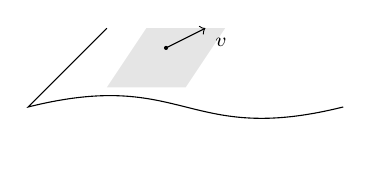
\begin{tikzpicture}%[xscale=.75]
    \draw (0,0) .. controls (-2,-.5) and (-2,.5) .. (-4,0) -- (-3,1);
    \begin{scope}[xshift=1cm,yshift=1cm]
    % \draw[fill=gray!10 draw=black] (0,0) .. controls (-2,-.5) and (-2,.5) .. (-4,0) -- (-3,1);
    % \draw[xshift=3cm, yshift=-1cm] (-4,0) -- (-3,1);
    \end{scope}
    \fill[xshift=-3cm,yshift=.25cm,gray!20, scale=.5] (0,0) -- (2,0) -- (3,1.5) -- (1,1.5) -- cycle;
    \fill (-2.25,.75) circle (.75pt);
    \draw[->] (-2.25,.75) -- +(.5,.25) node[below right] {\scriptsize $v$};
  \end{tikzpicture}
\end{document}